\chapter{Analysis Motivation and Methodology}
\label{ch:analysis_mnm}

This chapter will provide the underlying motivation for the main topic of this thesis, along with a high-level overview of the methodology used to perform the analysis. The core procedure of the analysis can be summarized with the phrase:
\begin{center}
\fbox{
    \centering
    \begin{minipage}{30em}
    \centering
    \textbf{Using two-particle h-\lmb angular correlations to investigate the production of strange quarks both in and out of jets in \pPb collisions}
\end{minipage}}
\end{center}
To those unfamiliar with the field of heavy-ion physics, this statement may seem like a jumble of words. The aim of this chapter is to 
First, the motivation for this analysis will be given in detail, emphasizing the importance of the \lmb baryon and why it was chosen for this study. Next, the main technique used to perform the analysis will be introduced, along with a brief overview of the analysis procedure. Finally, the main observables of interest will be mathematically defined to avoid any ambiguity in the following chapters.

\section{Motivation}
As mentioned in Section~\ref{sec:strangeness_enhancement}, the enhancement of strange quarks relative to non-strange ($u$ and $d$) quarks in heavy ion collisions is a key indicator of the production of a QGP. Experimentally, this enhancement is seen by measuring the production of strange hadrons ($\Lambda$, $K^0$, $\phi$, $\Xi$, $\Omega$) relative to the production of pions as a function of event multiplicity. The results of such measurements from the ALICE is shown again in Figure \ref{fig:ref_enhancement} for reference. 

\begin{figure}
\centering
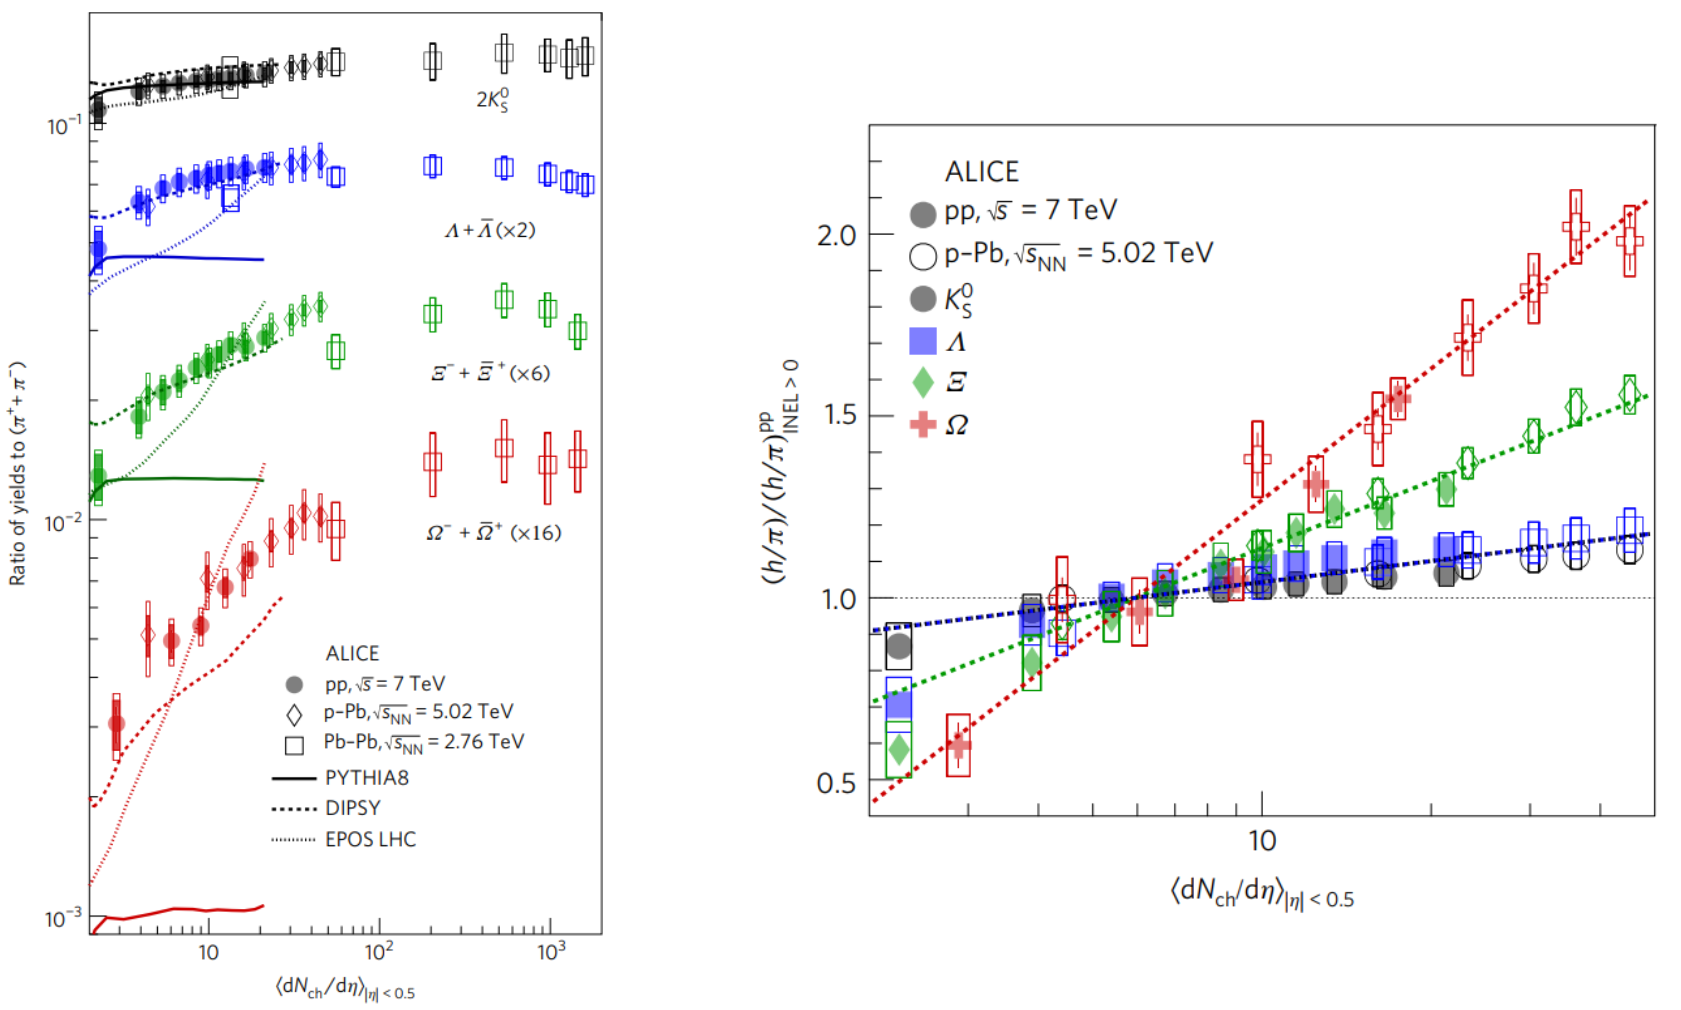
\includegraphics[width=\textwidth]{figures/introduction/strangeness_enhancement.png}
\caption{The enhancement of strange hadrons relative to pions as a function of event multiplicity in \PbPb collisions at $\sqrt{s_{NN}} = 2.76$ TeV. Taken from \cite{ALICE:2017jyt}.}
\label{fig:ref_enhancement}
\end{figure}

This figure shows a clear indication of an \textit{onset} of strangeness enhancement, which transitions smoothly from low multiplicity pp to high multiplicity Pb--Pb in a way that is independent of collision system. While statistical models are able to well-describe these particle ratios in low multiplicity pp (in the form of a canonical ensemble without chemical equilibriation~\cite{NATURE15, NATURE16}) and high multiplicity Pb--Pb (in the form of a grand canonical ensemble~\cite{NATURE16}), such models cannot describe the transition region. Phenomenological extensions to these models are able to produce a smooth transition between the two regimes~\cite{NATURE18, NATURE19}, but the microscopic origins of this observed enhancement are still unkown. 

This thesis aims to shed light on these origins by investigating this enhancement in different kinematic regimes. In particular, the production of strangeness within the near-side and away-side components of dijets\footnote{For more details see Section~\ref{sec:jet_quenching} in the introduction.} will be studied and compared with the strangeness production outside of the dijet system. The production in the near-side component of the dijet corresponds to unmodified strange quark production in a jet, whereas the away-side production corresponds to strangeness production in a jet whose initial partons traversed through the QGP medium. The production outside of the dijet system is meant to represent the production of strangeness in the QGP medium itself, and serves as a baseline for ``soft'' quark production. Measuring the strangeness production in these regions can be used to determine their relative contributions to the overall observed enhancement, in turn illuminating some of its origins at a fundamental level.

The p--Pb collision system is ideal for this study for two major reasons. The first is that the p--Pb system captures the \textit{entirety} of the observed onset of strangeness enhancement, as seen in Figure~\ref{fig:ref_enhancement}. Thus when trying to \textit{study} this onset, \pPb collisions are the most natural choice. The second reason is that pp collisions give rise to a large amount of jet-like production, with very little medium-like production. Pb--Pb collisions, on the other hand, are dominated by medium-like production with very little jet-like contributions. The p--Pb system produces a healthy blend of both jet- and medium-like production, making it the ideal candidate for analyzing the production of strangeness in these two regimes.

\subsection{The \lmb baryon}
\label{sec:lambda_baryon}

When studying strange quark production in experiment, a choice of strange hadron must be made. In this thesis, the strange hadron of choice is the \textbf{lambda baryon} (\lmb). The \lmb is a neutral hadron with mass $1.116$ \GeVmass, consisting of one up, one down, and one strange quark ($uds$). The reasons for choosing the \lmb baryon for this analysis are as follows.

Firstly, it is the lightest baryon containing a strange quark, and is thus the most abundantly produced strange baryon in high energy particle collisions. This makes it an ideal candidate for differential studies like the one presented in this thesis, as correlation measurements require a \textit{lot} of statistics. Second, the \lmb has a very long lifetime--relative to the collision evolution--as it can only decay weakly. This has two effects:
\begin{enumerate}
    \item \lmb baryons produced early on in the collision survive until the end of the collision, keeping their decay products in-tact. This is not the case for strongly decaying resonace states like the $K^*$, which often decay within the hadronic gas phase of the collision. This can result in their decay products ``rescattering'' off other hadrons within the gas~\cite{Rescatter}, making it impossible to reconstruct the original resonance.
    \item The \lmb often travels a significant distance before decaying, which allows for the reconstruction of its decay vertex in the detector. This substantially reduces the background contribution to the \lmb signal, which is discussed in more detail in Section~\ref{sec:v0_decay}
\end{enumerate}
Furthermore, the integrated production of \lmb baryons relative to pions has been studied extensively in pp, p--Pb and Pb--Pb collisions at ALICE, as shown in Figure~\ref{fig:lambda_enhancement}. Due to its strange quark content, the \lmb/pion ratio exhibits a large enhancement, especially in the p--Pb region. The measurements in Figure~\ref{fig:lambda_enhancement} serve as a baseline for the differential studies presented in this thesis.

\begin{figure}
\centering
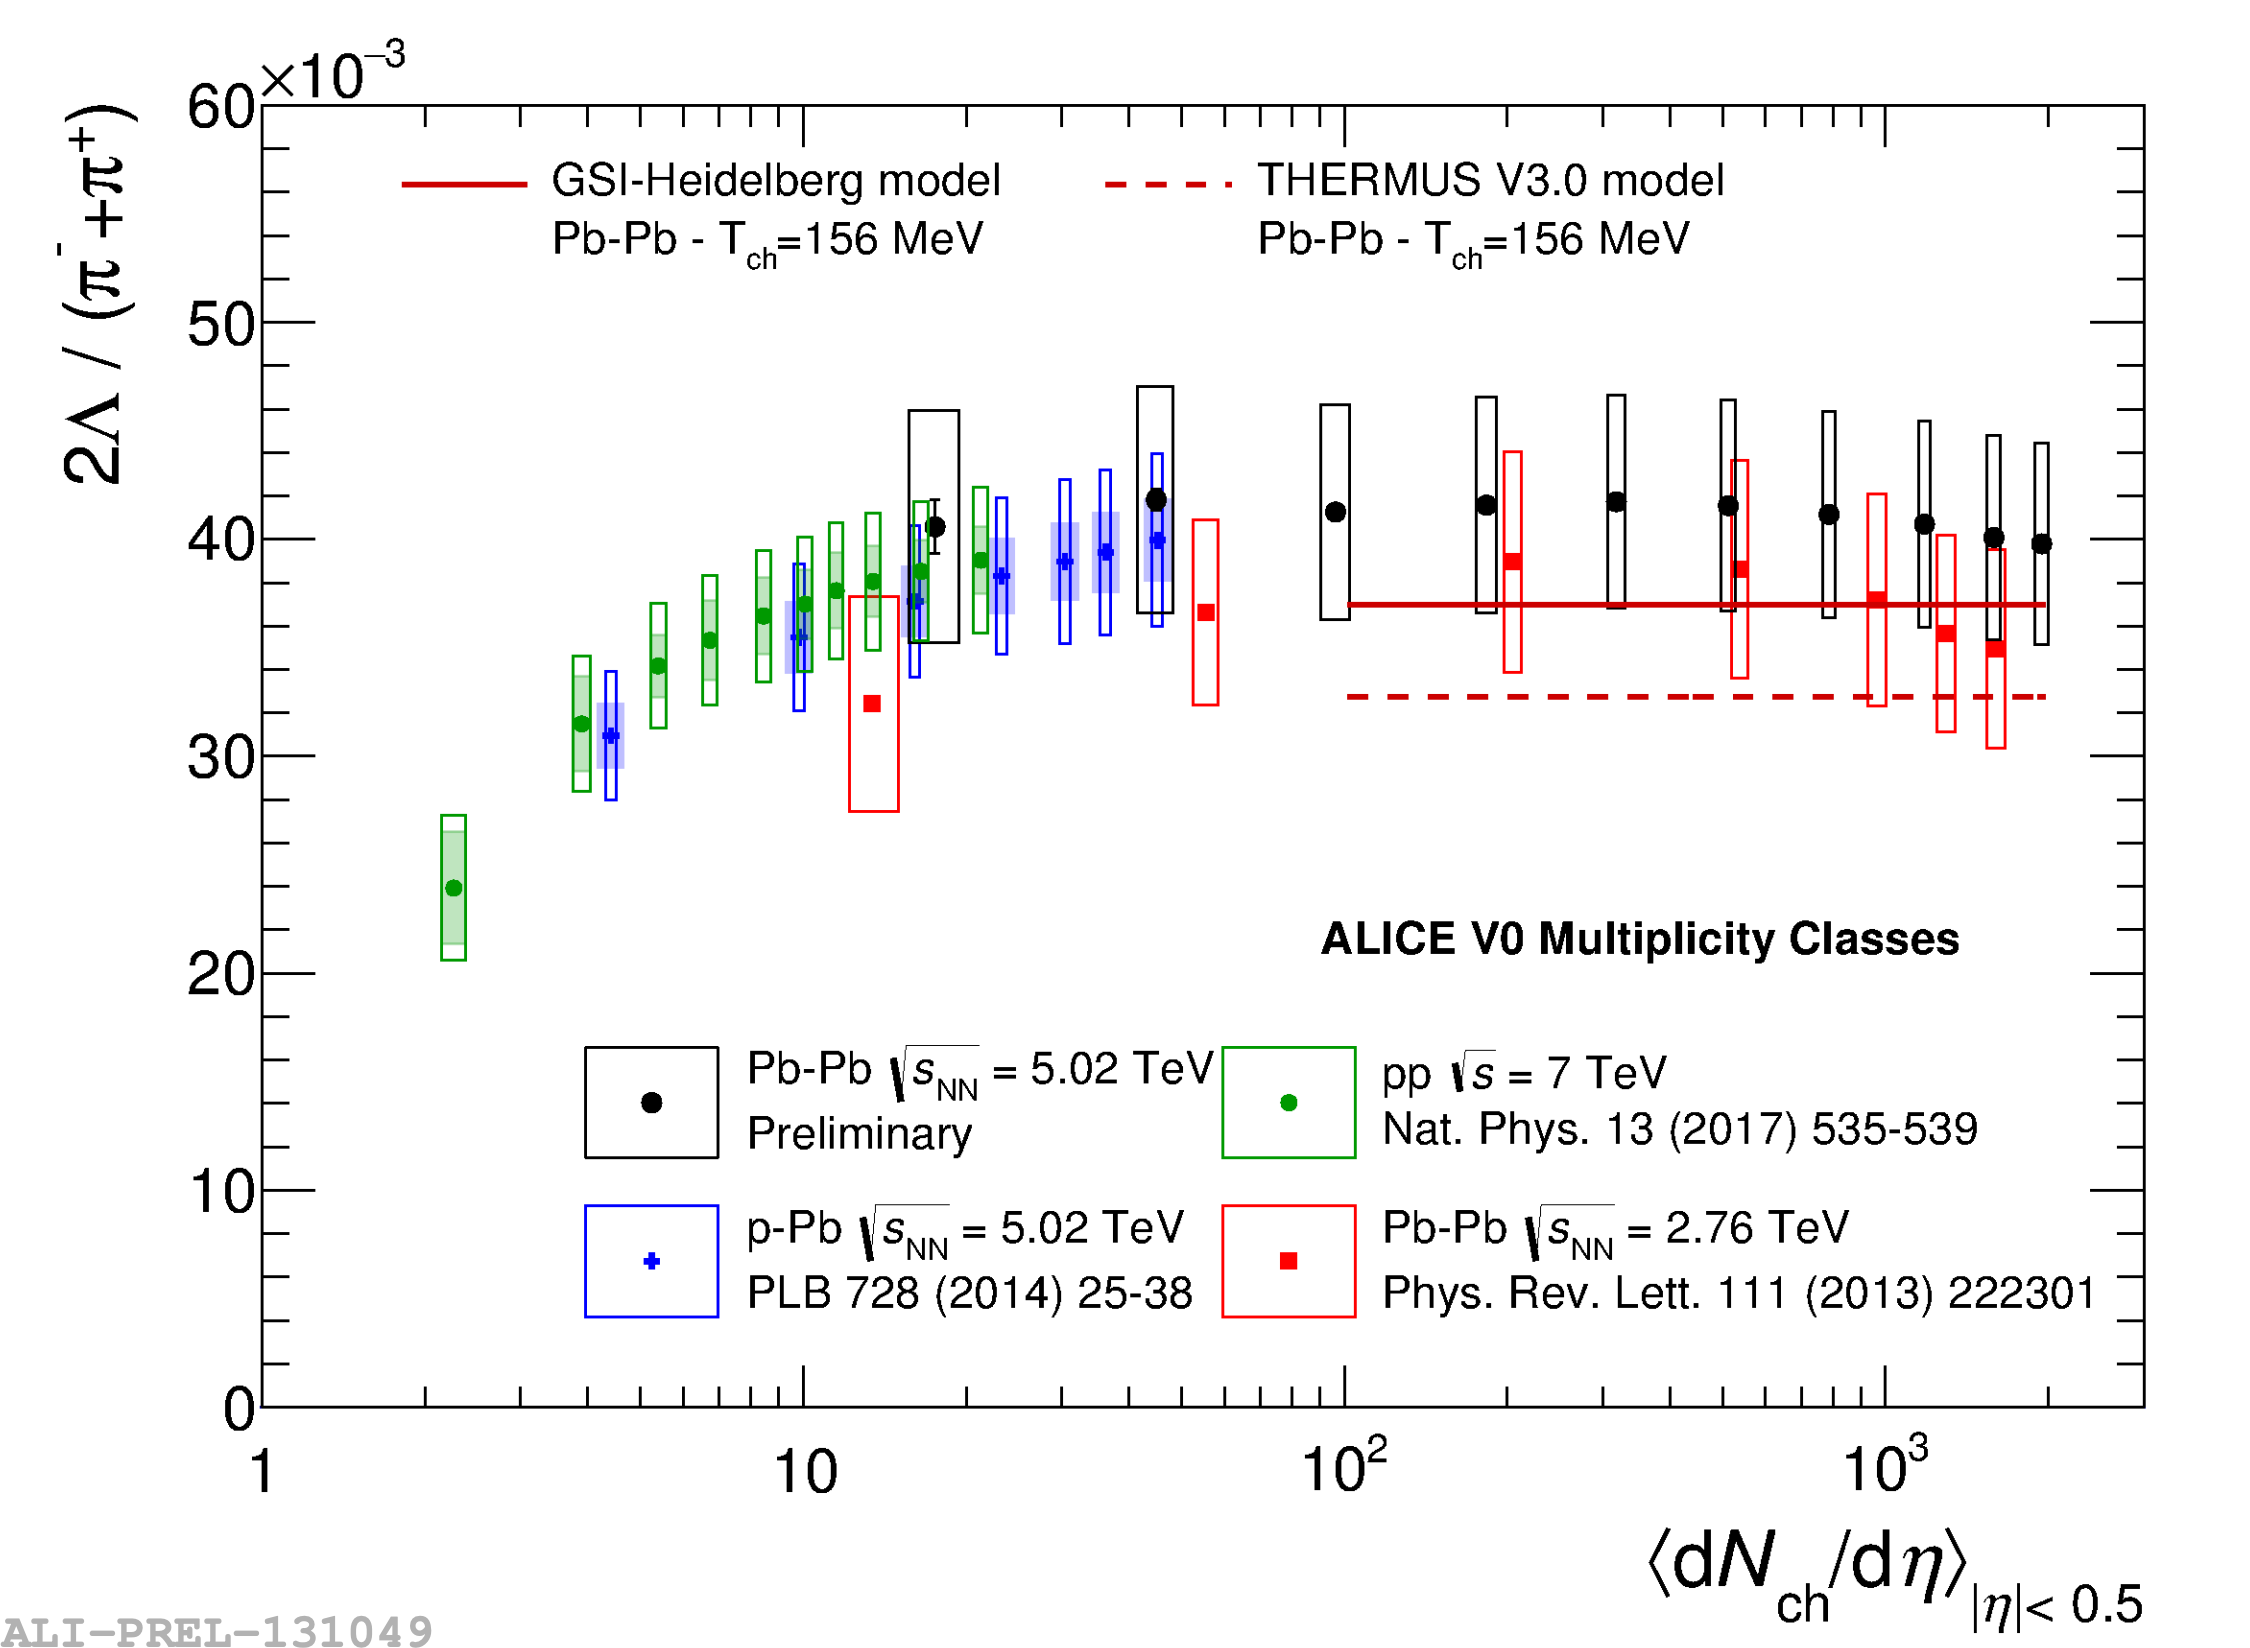
\includegraphics[width=\textwidth]{figures/mnm/lambda_enhancement.png}
\caption{The \pt-integrated \lmb/pion ratio as a function of event multiplicity in pp, p--Pb, and Pb--Pb collisions at ALICE, taken from \cite{LambdaEnhancement}.}
\end{figure}

Finally, the \lmb baryon, with a net strangeness of one, shares a similar mass with the $\phi(1020)$ resonance ($s\bar{s}$), which has a net strangeness of zero. Thus the differences between ``open'' strangeness ($|S| > 0$) and ``hidden'' strangeness ($|S| = 0$) can be studied by comparing the production of \lmb baryons with the production of $\phi$ resonances. Due to their similar masses, any changes in the production of these two hadrons due to differing masses would be negligible.

\section{Methodology}

\subsection{The main technique}
To separate the production of \lmb baryons into the jet and non-jet regions, \textbf{two-particle angular correlations} are used. By looking at the relative azimuthal angles $\Delta\varphi = \varphi_{\text{trigger}} - \varphi_{\text{associated}}$ between a high momentum \textbf{trigger} particle and a lower momentum \textbf{associated} particle, the resulting distribution can be used to separate the production of the associated particles into distinct regions. These regions can be seen in Figure~\ref{fig:dphi_cartoon}, and will be reffered to as
%
\begin{itemize}
\item the \textbf{near-side region} shown in red, corresponding to near-side jet production with no medium interactions, 
\item the \textbf{away-side region} shown in blue, corresponding to away-side jet production with possible medium interaction, and
\item the \textbf{underlying event (UE) region} shown in green, corresponding to the uncorrelated production within the medium.
\end{itemize}
%
\begin{figure}
\centering
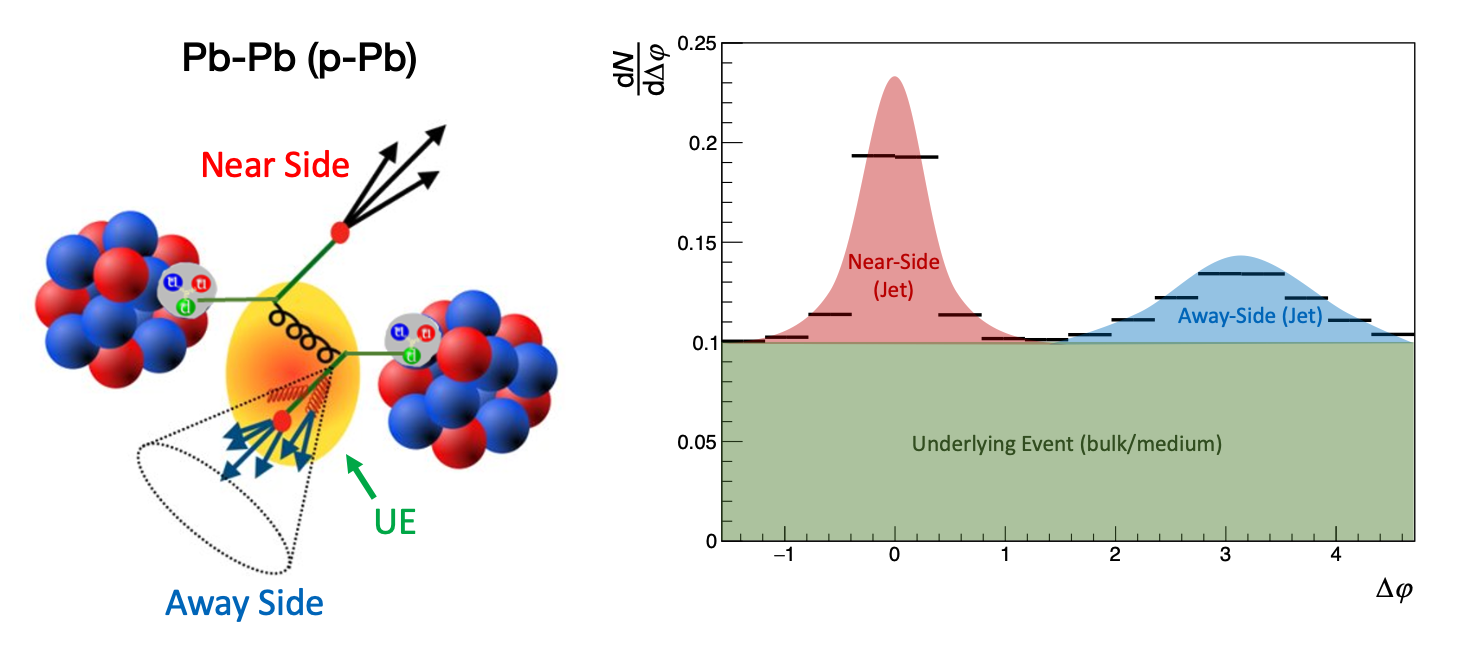
\includegraphics[width=\textwidth]{figures/mnm/dphi_cartoon.png}
\caption{A cartoon of a Pb--Pb (p--Pb) collision that produces particles in the near- and away-side jets, along with the UE. The the corresponding regions in the $\Delta\varphi$ distribution are highlighted on the right.}
\label{fig:dphi_cartoon}
\end{figure}

The clear separation between these regions in the $\Delta\varphi$ distribution can be understood from the following argument. If the trigger momentum is high enough ( $>$ 4 GeV/$c$), it must be closely aligned with the near-side jet axis~\cite{JetAxisArgument}. As such, the associated particles that are produced in the near-side of the jet will have a small relative angle to the trigger, near $\Delta\varphi = 0$. The associated particle production in the away-side jet would then be 180$^\circ$ away from the trigger, near $\Delta\varphi = \pi$. Finally, the uncorrelated\footnote{Elliptic flow ($v_2$) gives rise to a small correlation across $\Delta\varphi$, see Section~\ref{sec:collective_flow}.} associated particle production within the medium would be randomly distributed across $\Delta\varphi$, manifesting as a (mostly) flat background for which the near- and away-side peaks sit on top of. 

\subsection{The end goal}

In this thesis, the h-\lmb $\Delta\varphi$ distributions in p--Pb collisions at the ALICE detector will be measured across a wide range of multiplicities. The resulting distributions will be used to extract the associated \lmb yields in each of the near-side, away-side and UE regions. Moreover, the correlation distributions will be used to extract the widths of the near- and away-side jet peaks, which aid in the study of the effects of jet-medium interactions on the production of strange hadrons~\cite{DeepaPaper, DPaper}. Each of these observables will be compared with those of a h-h (dihadron) sample, which serves as a proxy for non-strange quark (pion) production. These measurements will be compared with theoretical model predictions from the event generators detailed in Section~\ref{sec:models}. The differences between open and hidden strangeness production will also be explored using previously published h-$\phi(1020)$ angular correlation measurements in \pPb collisions~\cite{JustinPaper}. 

Because the analysis procedure is dense with technical details, the remainder of this chapter will be dedicated to providing a high-level overview of the analysis. The specifics of the analysis procedure will be discussed in Chapter~\ref{ch:analysis_details}.

\subsection{A brief overview of the analysis}
\label{sec:analysis}

To get to the final h-\lmb and h-h $\Delta\varphi$ distributions of interest, a correlation function must be specified. There are a multitude of ways to define such correlation functions~\cite{CorrelationFunction}, but this thesis uses the per-trigger normalized associated particle yield,
\begin{equation}
    C_{\text{yield}}(\Delta\varphi, \Delta\eta) = \frac{1}{N_{\text{trig}}}\frac{d^2N_{\text{pair}}}{d\Delta\varphi d\Delta\eta}.
\label{eq:corr}
\end{equation}
Note that this is a 2D distribution, which has information about the angular separation in both $\Delta\varphi$ \textit{and} $\Delta\eta$. Due to the finite acceptance of the detector along $\eta$, na\"ively integrating over $\Delta\eta$ (in other words, just looking at the angular separation in $\Delta\varphi$) would introduce a bias in the jet components, which will be discussed in Section~\ref{sec:mixed_event}. As mentioned previously, the angular separations $\Delta\varphi$ and $\Delta\eta$ are measured between a high momentum trigger hadron (h)--which serves as a proxy for the jet axis--and a lower momentum associated hadron ($\Lambda$ or h). 

\subsubsection{Raw distribution corrections}
Unfortunately, the correlation function given by Equation~\ref{eq:corr} cannot be obtained without a series of corrections to the raw distribution for various detector effects. The \textbf{raw distribution} is defined as the distribution obtained by counting the number of observed trigger-associated pairs within a given event, summed up over the entire event sample. The corrected distribution is then given by
%
\begin{equation}
    C_{\text{yield}}(\Delta\varphi, \Delta\eta) = \frac{1}{N_{\text{trig}}^{\text{corr}}}\frac{1}{\epsilon_{\text{trig}}\times\epsilon_{\text{assoc}}}B(0,0)\frac{S(\Delta\varphi, \Delta\eta)}{B(\Delta\varphi, \Delta\eta)}\frac{1}{\epsilon_{\text{pair}}(\Delta\varphi, \Delta\eta)},
\label{eq:corr_detector}
\end{equation}
%
where $S(\Delta\varphi, \Delta\eta)$ is the aforementioned raw distribution. $N_{\text{trig}}$ is the total number of trigger hadrons across the event sample, corrected for trigger efficiency. Each of $\epsilon_{\text{trig}}$, $\epsilon_{\text{assoc}}$ and $\epsilon_{pair}$ are efficiency correction factors that are discussed in more detail within Section~\ref{sec:single_particle_corr}.  $B(\Delta\varphi, \Delta\eta)$ is the distribution generated by combining trigger and associated particles that are produced in \textit{separate} events, called the ``mixed-event'' distribution. A simple diagram showing the differences between the generation of $S(\Delta\varphi, \Delta\eta)$ and $B(\Delta\varphi, \Delta\eta)$ is shown in Figure~\ref{fig:mixed_event_cartoon}. This distribution is used to correct for the finite acceptance of the detector, and is detailed in Section~\ref{sec:acceptance_corr}.

\begin{figure}
\centering
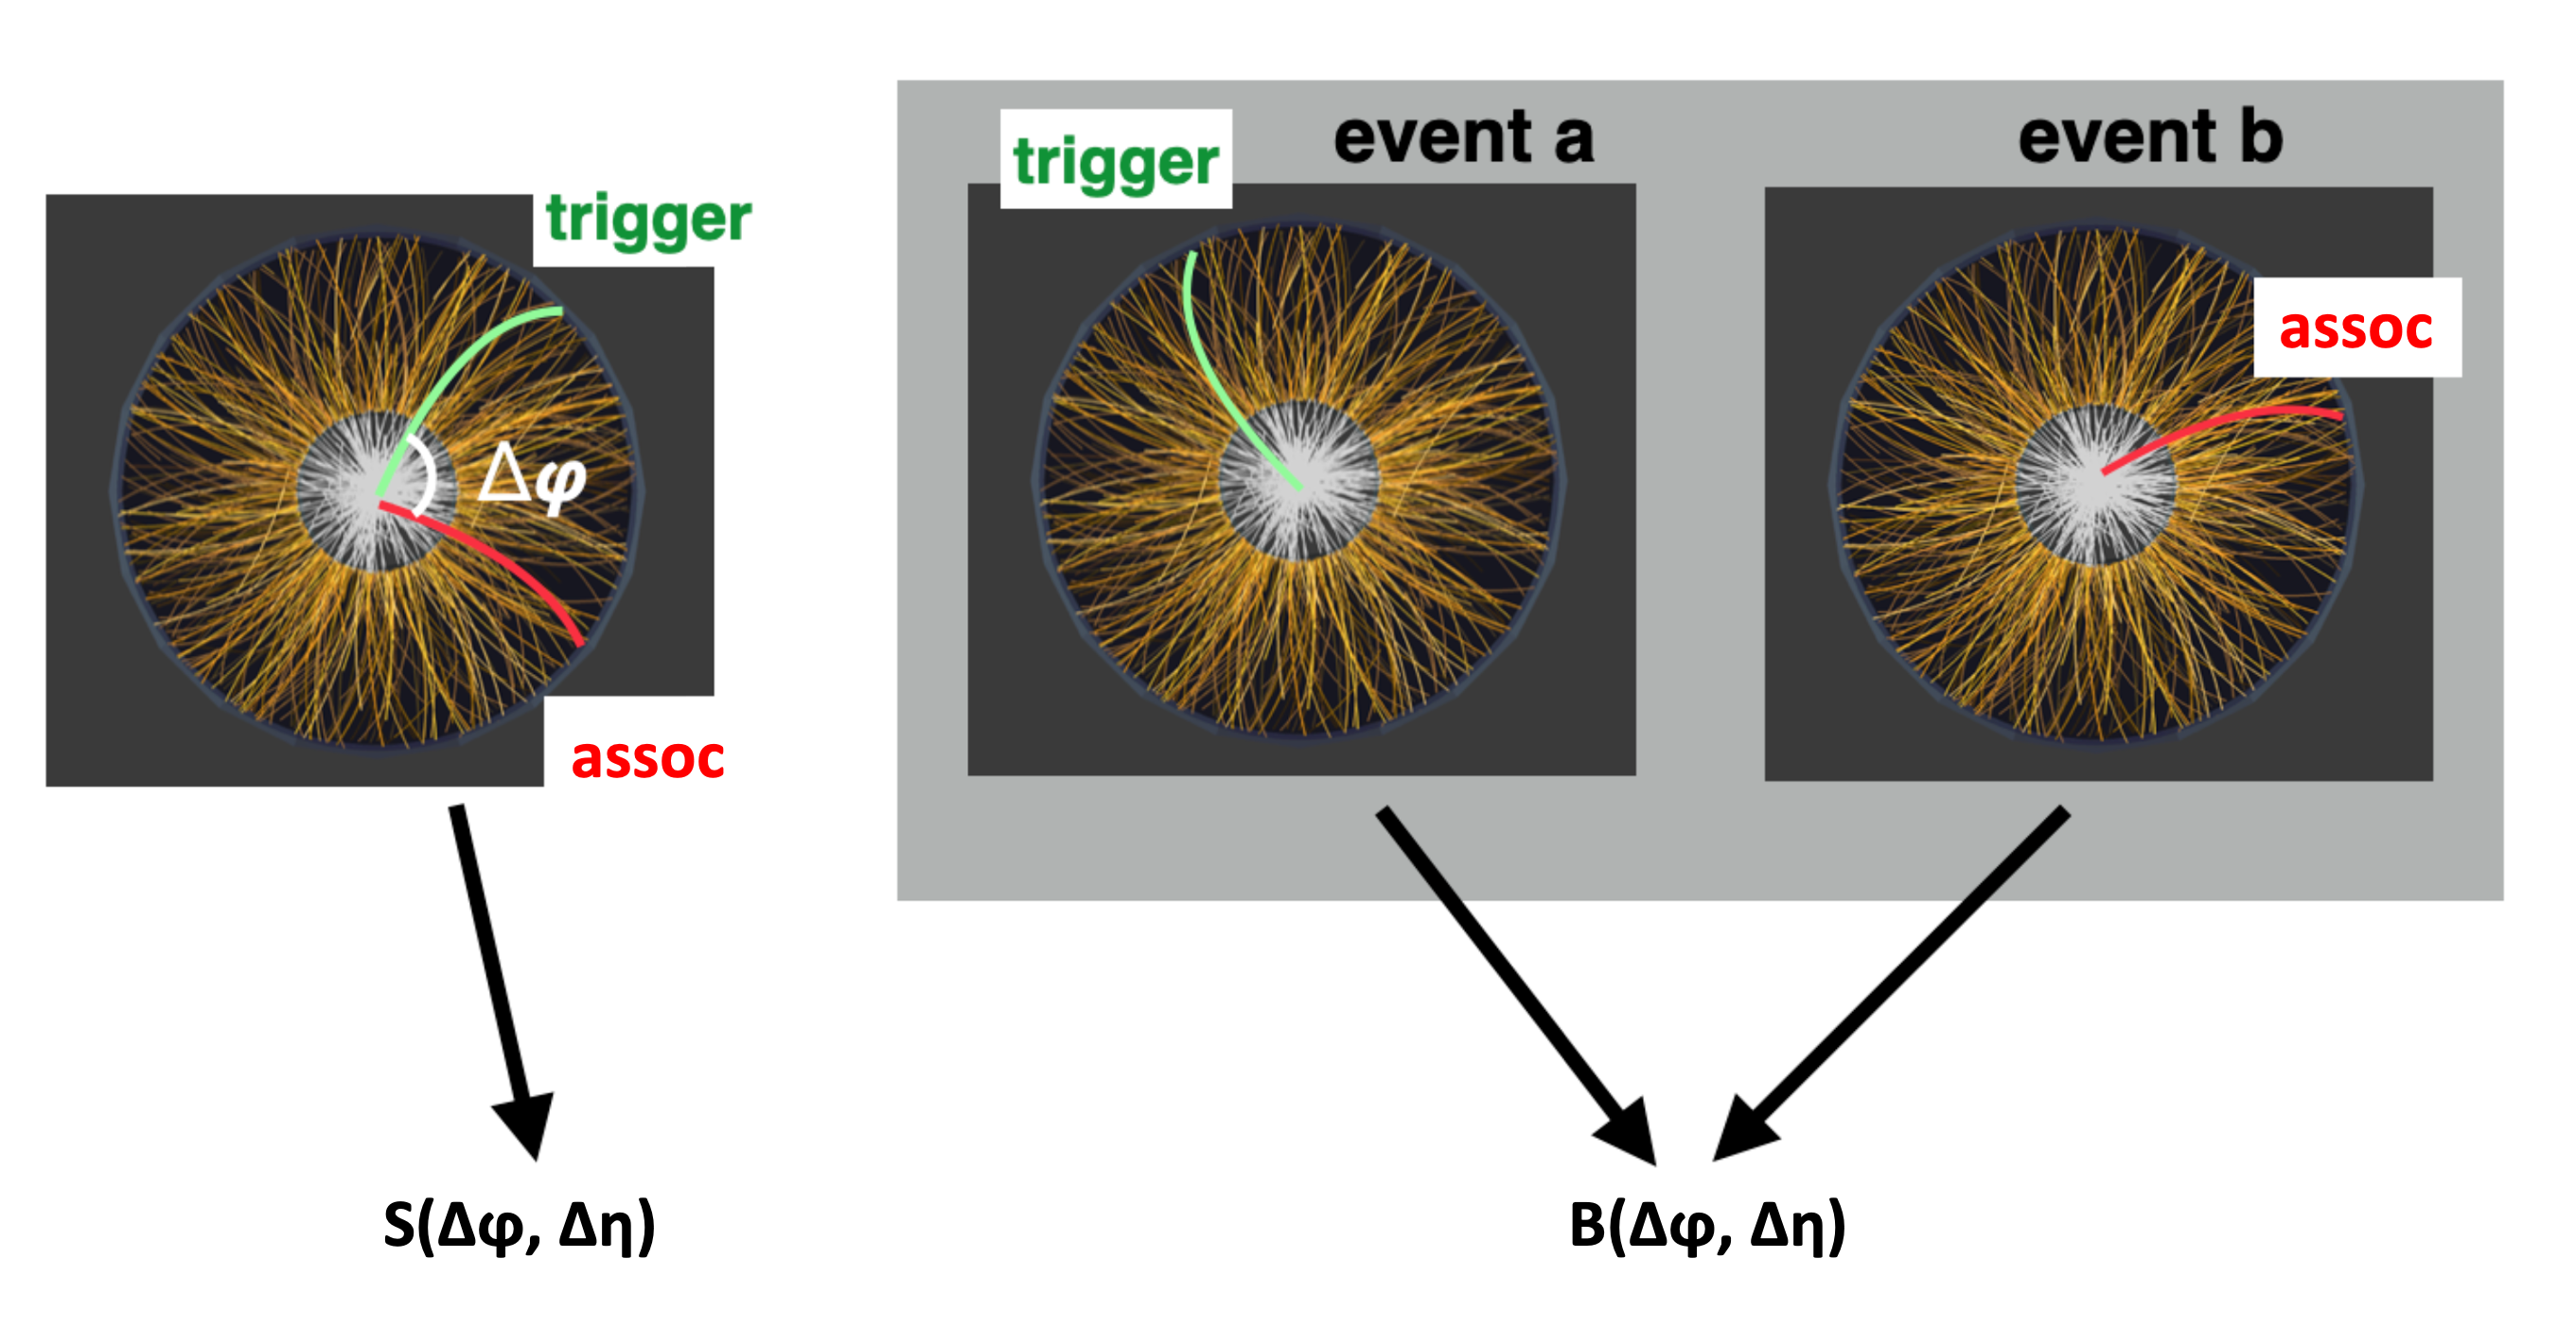
\includegraphics[width=\textwidth]{figures/mnm/mixed_event_cartoon.png}
\caption{A simple diagram showing the differences between the generation of the raw distribution $S(\Delta\varphi, \Delta\eta)$ (left) and the mixed-event distribution $B(\Delta\varphi, \Delta\eta)$ (right). The yellow tracks are those observed by the detector. The raw distribution is obtained by looking at trigger-associated pairs within the same event, whereas the mixed-event distribution is generated from pairs that come from separate events. Note that both $\Delta\varphi$ and $\Delta\eta$ cannot be easily shown on a 2D plot, but the distributions are filled with both quantities.}
\label{fig:mixed_event_cartoon}
\end{figure}

Examples of $S(\Delta\varphi, \Delta\eta)$, $B(\Delta\varphi, \Delta\eta)$ and $C_{\text{yield}}(\Delta\varphi, \Delta\eta)$ for h-\lmb pairs can be found in Figure ~\ref{fig:twod_cor}. The peaks observed around $\Delta\varphi = 0$ and $\Delta\varphi = \pi$ in the fully corrected correlation function define the aforementioned near- and away-side regions, respectively, which lie on top of the uncorrelated UE.

\begin{figure}[t]
\makebox[\linewidth][c]{%
\centering
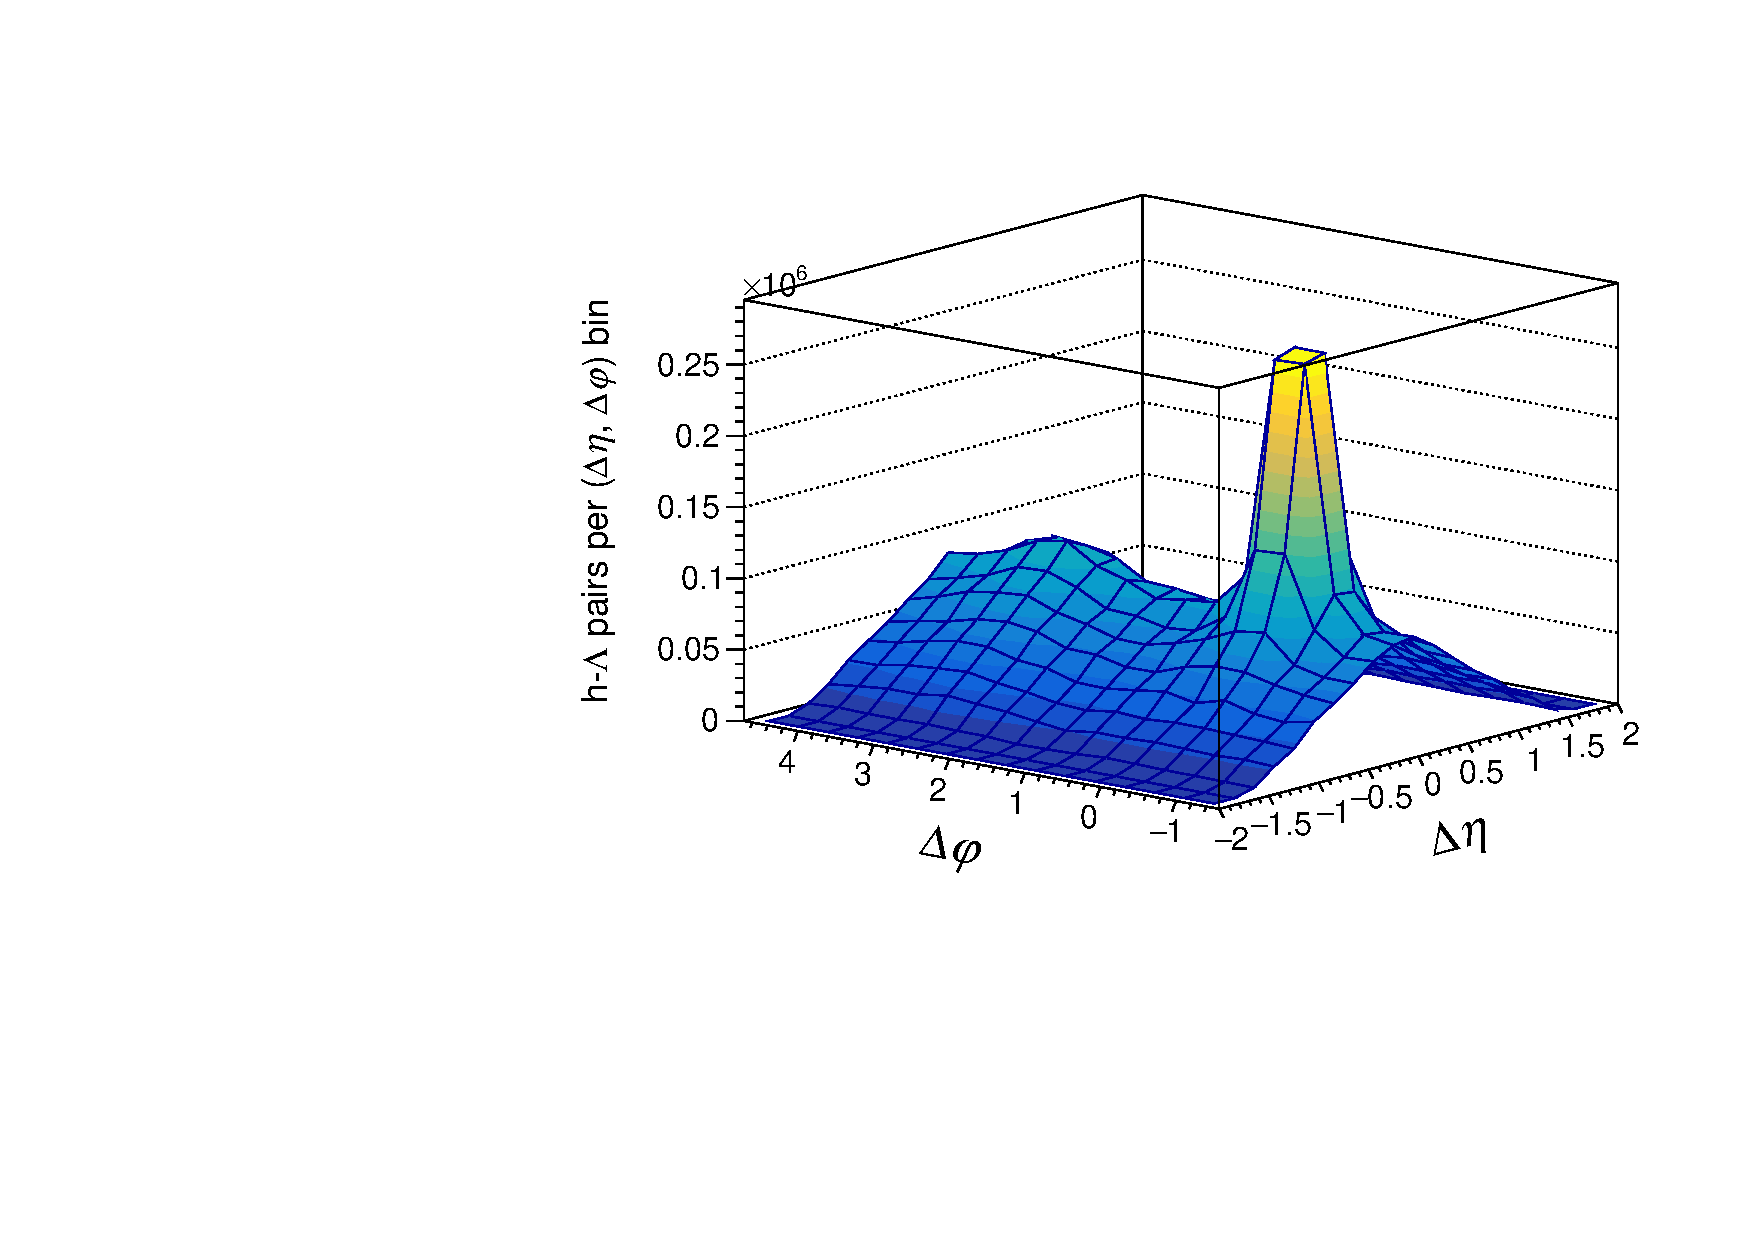
\includegraphics[width=0.35\textwidth]{figures/mnm/h_lambda_2d_nomixcor_20_50_highpt.pdf}
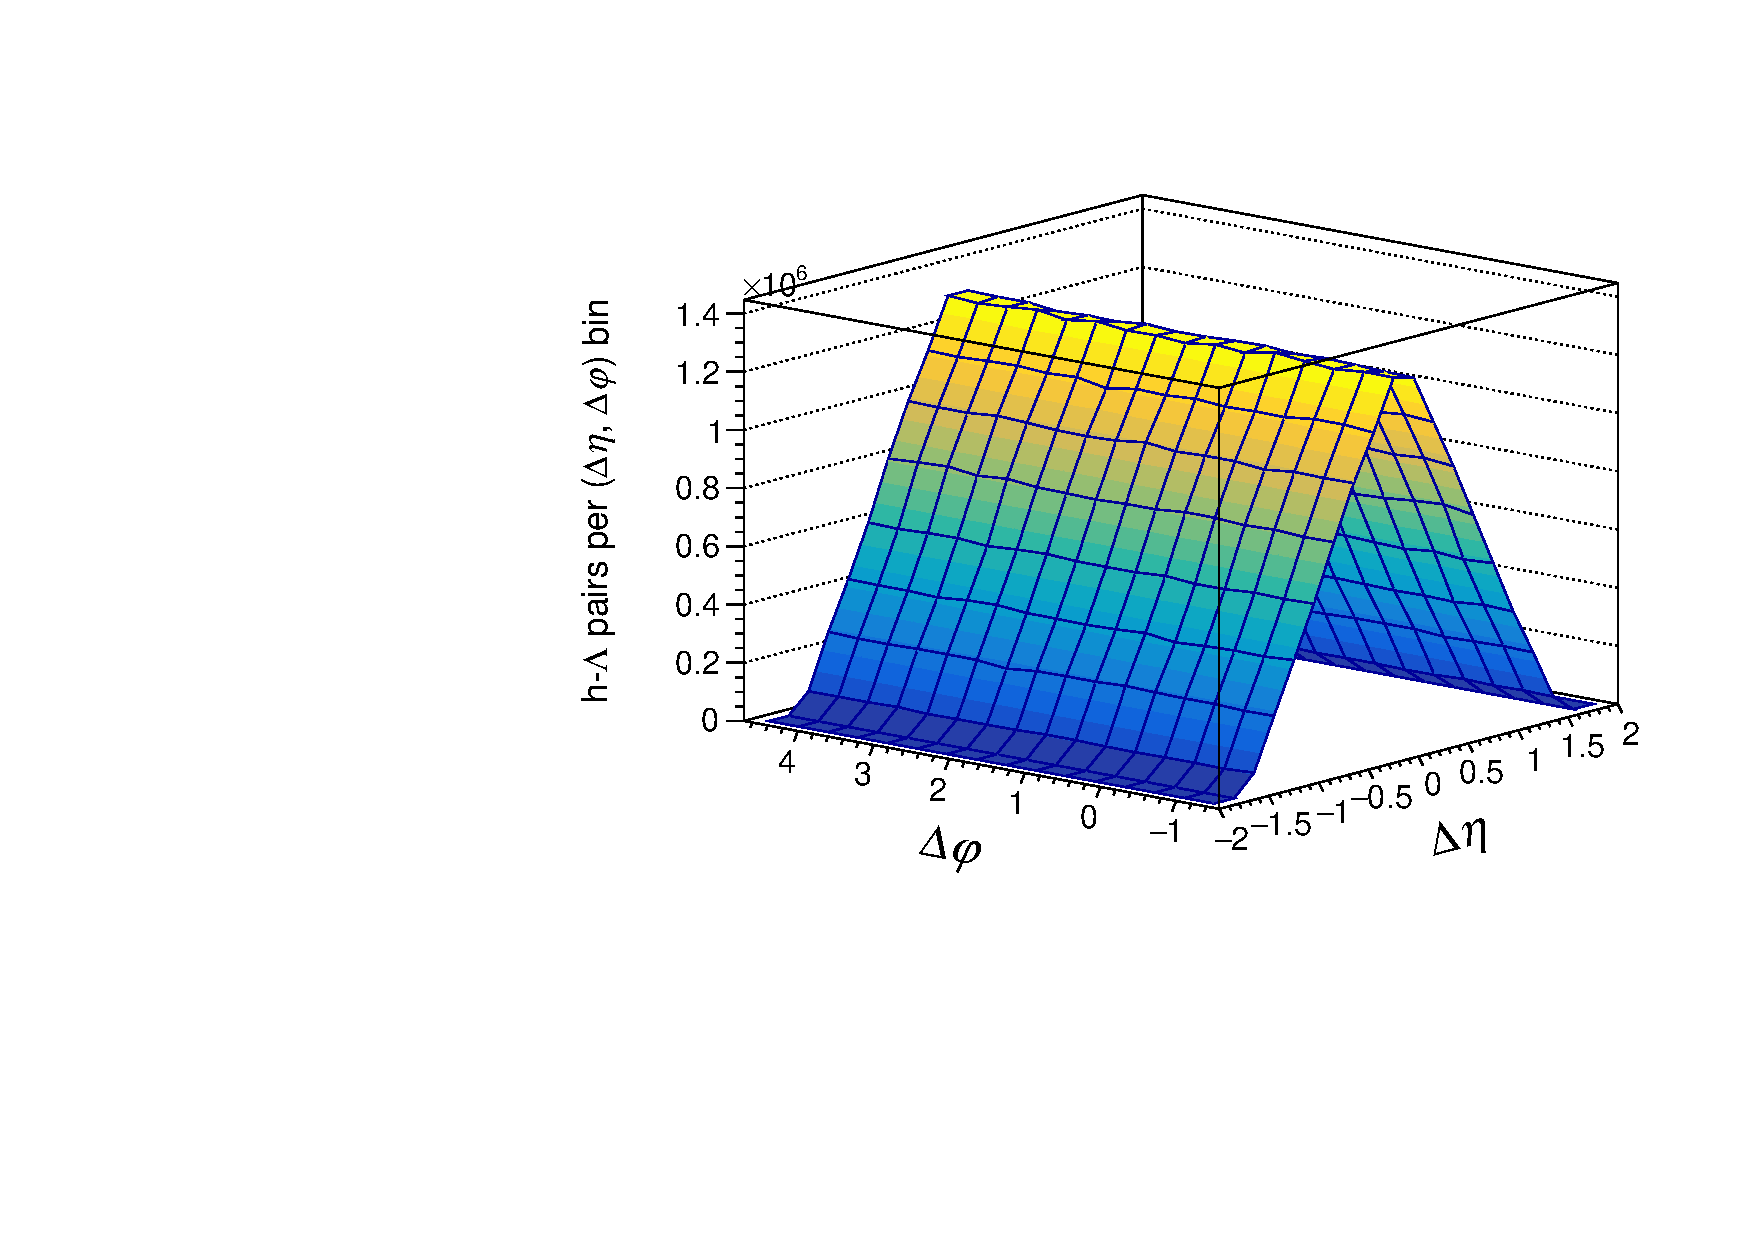
\includegraphics[width=0.35\textwidth]{figures/mnm/h_lambda_2d_mixed_20_50_highpt.pdf}
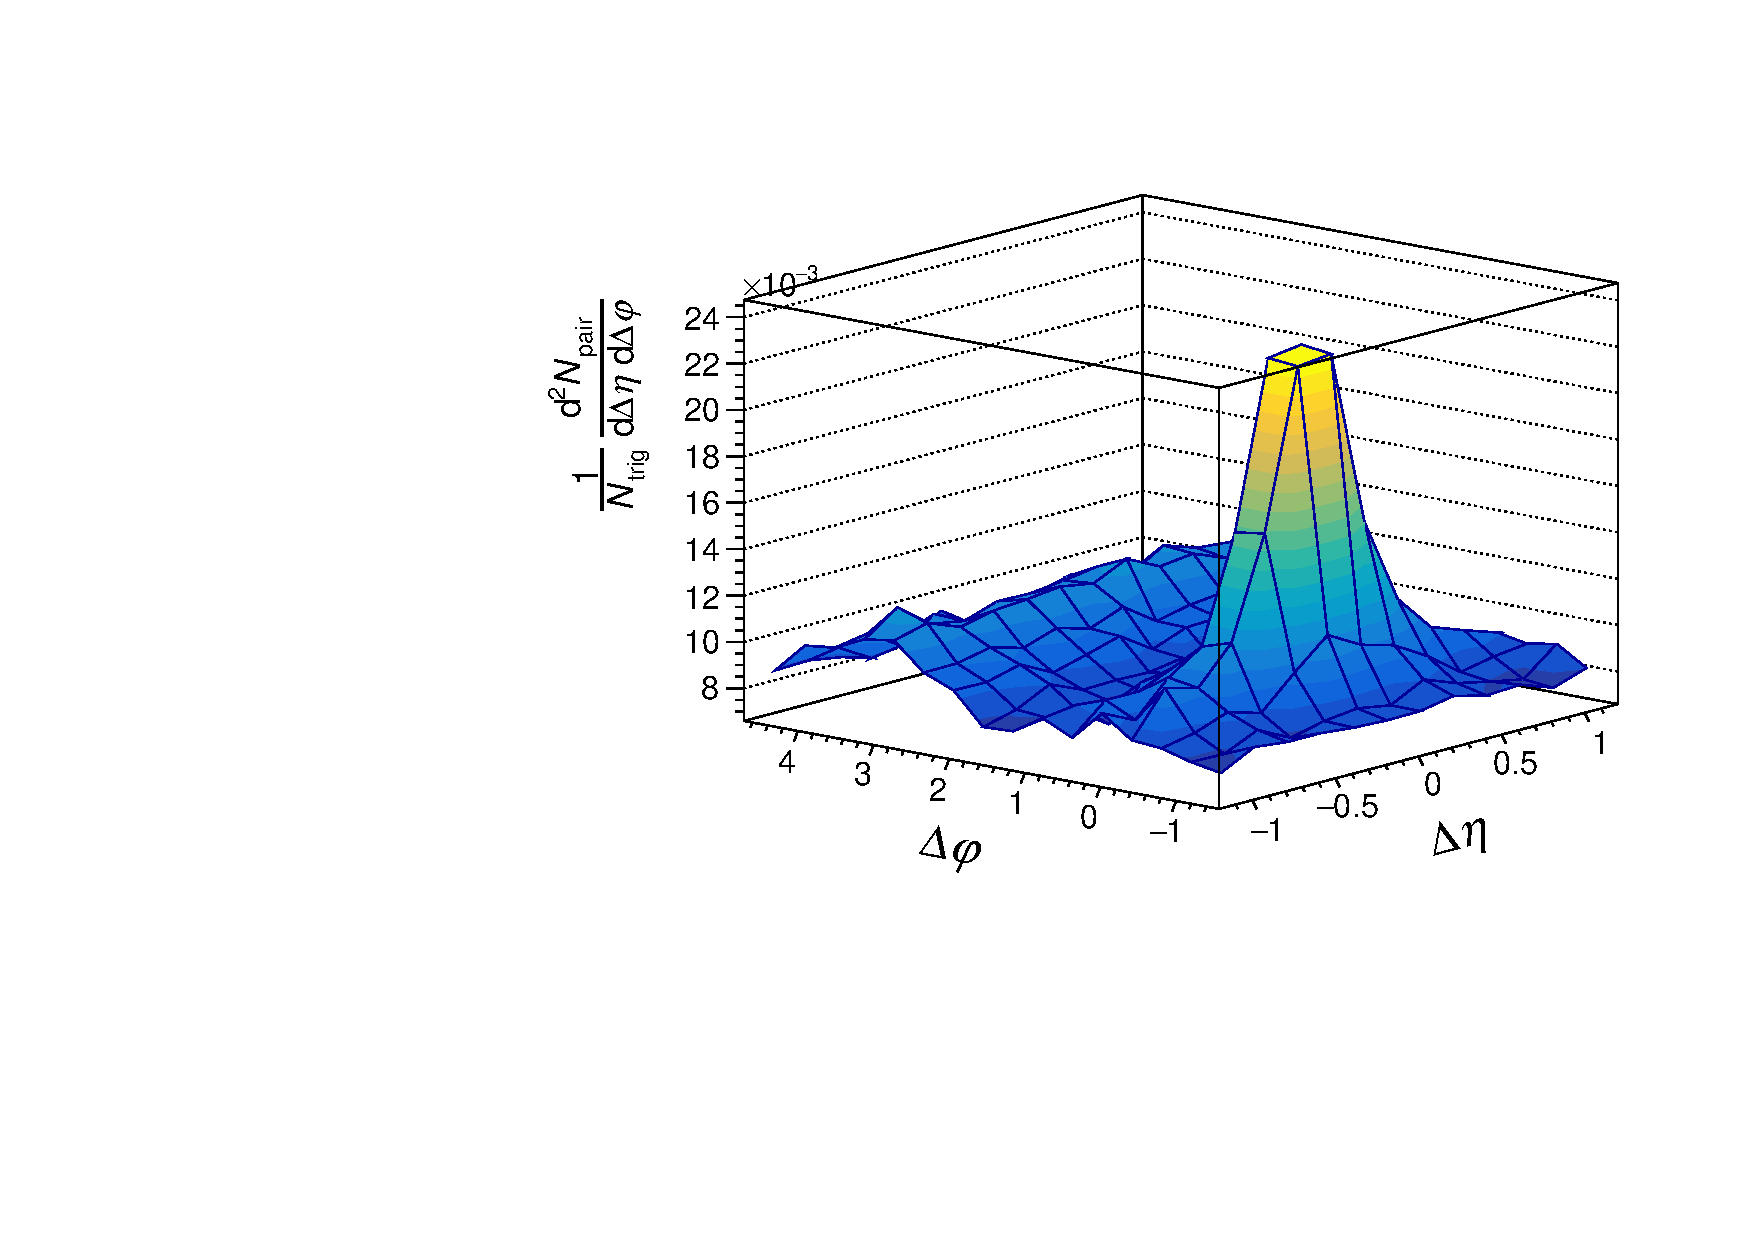
\includegraphics[width=0.35\textwidth]{figures/mnm/h_lambda_2d_mixcor_20_50_highpt.pdf}
}
\caption{Examples of the h-\lmb same-event distribution $S(\Delta\varphi, \Delta\eta)$ (left), mixed-event distribution $B(\Delta\varphi, \Delta\eta)$ (middle), and fully corrected correlation function $C_{\text{yield}}(\Delta\varphi, \Delta\eta)$ (right).}
\label{fig:twod_cor}
\end{figure}

\subsubsection{Underlying event fit}
\label{sec:uefit}

Once all of the corrections have been applied to the raw distributions, the resulting correlation function $C_{\text{yield}}(\Delta\varphi, \Delta\eta)$ can be projected onto $\Delta\varphi$ to obtain the 1D distribution $dN/d\Delta\varphi$. To extract the near- and away-side widths and the per-trigger yields in each kinematic region from these distributions, the underlying event contribution $U(\Delta\varphi$) must be quantified. While there are multiple ways to do this, the nominal procedure is simply to fix $U(\Delta\varphi)$ to the average of the $\Delta\varphi$ distribution in the regions where there is little-to-no jet contribution. Explicitly, these regions are 
\begin{itemize}
\item $(-\frac{\pi}{2}, -\frac{\pi}{4})$, 
\item $(\frac{\pi}{4}, \frac{5\pi}{8})$, and
\item $(\frac{11\pi}{8}, \frac{3\pi}{2})$. 
\end{itemize}
The effects of varying these regions, along with other assumptions of the form of $U(\Delta\varphi)$, are explored in detail wthin Chapter~\ref{ch:systematics}.

\subsubsection{Yield and width extraction}
 After obtaining the underlying event fit $U(\Delta\varphi)$, the associated particle yields in the jet-like and UE regions are extracted using
 %
\begin{eqnarray}
    Y_{\text{near}} = \int_{-\pi/2}^{\pi/2} (\frac{dN}{d\Delta\varphi}- U(\Delta\varphi))d\Delta\varphi,  \  \ Y_{\text{away}} = & \int_{\pi/2}^{3\pi/2} (\frac{dN}{d\Delta\varphi}- U(\Delta\varphi))d\Delta\varphi 
    \label{eq:jet_yields}
    \\ 
    Y_{\text{UE}} = \int_{-\pi/2}^{3\pi/2} U(\Delta\varphi)d\Delta\varphi,
\label{eq:ue_yield}
\end{eqnarray}
%
where the subscripts near, away and UE refer to the near-side, away-side, and underlying event regions, respectively.

In order to quantify the widths of the near- and away-side peak regions, the $\Delta\varphi$ distributions are fit using the function
%
\begin{equation}
    F(\Delta\varphi) = U(\Delta\varphi) + \frac{e^{\kappa_{\text{near}}\text{cos}(\Delta\varphi - \mu_{\text{near}})}}{2\pi I_0(\kappa_{\text{near}})} + \frac{e^{\kappa_{\text{away}}\text{cos}(\Delta\varphi - \mu_{\text{away}})}}{2\pi I_0(\kappa_{\text{away}})},
\label{eq:fullfit}
\end{equation}
%
which is composed of two von Mises functions describing the near- and away-side peaks. Von Mises functions~\cite{VonMises1, VonMises2} are the circular analogs of Gaussian distributions and provide the best fit to the $2\pi$-periodic $\Delta\varphi$ distributions. The $\kappa_{\text{near}}$ and $\kappa_{\text{away}}$ terms are the measure of the collimation of the near- and away-side peaks, respectively, and $I_{0}$ is the zeroth-order modified Bessel function. The underlying event fit $U(\Delta\varphi)$ is fixed to the function obtained from the previous section during fitting. Due to symmetry considerations, the means $\mu_{\text{near}}$ and  $\mu_{\text{away}}$ are also fixed to $0$ and  $\pi$, respectively. The width of the peaks is then quantified via~\cite{VonMises1}
%
\begin{equation}
    \sigma_{\text{near,away}} = \sqrt{-2\log\frac{I_1(\kappa_{\text{near,away}})}{I_0(\kappa_{\text{near,away}})}},
\label{eq:width}
\end{equation}
%
where $I_1$ is the first-order modified Bessel function and $\log(x)$ is the natural logarithm of $x$. Again, the effects of different choices for $F(\Delta\varphi)$ are detailed in Chapter~\ref{ch:systematics}.